\chapter{Полнотекстовый поиск с использованием Sphinx}\label{chap:sphinx} % Case Study: Sphinx-based Search

\footnotehref{http://sphinxsearch.com/}{Sphinx} --- это сервер полнотекстового поиска, благодаря которому реализован поиск на многих сайтах, включая сайт самого Yesod. Код, необходимый для интеграции Sphinx и Yesod довольно краток, но, в то же время, он затрагивает несколько непростых моментов, а потому является прекрасной иллюстрацией того, как использовать некоторые детали внутреннего устройства Yesod. % a great case study in how to play with some of the under-the-surface details of Yesod.

По существу нам предстоит реализовать три вещи: % There are essentially three different pieces at play here:

\begin{itemize}
  \item Сохранение данных, по которым мы хотели бы вести поиск. Для этого используется довольно незатейливый код Persistent, и мы не будем подробно останавливаться на этом моменте. % This is fairly straight-forward Persistent code, and we won't dwell on it much in this chapter.
  \item Доступ из Yesod к результатам поиска Sphinx. На самом деле, благодаря пакету \footnotehref{http://hackage.haskell.org/package/sphinx}{sphinx}, это довольно просто.
  \item Предоставление содержимого документов серверу Sphinx. Вот, где происходят интересные вещи! Вы узнаете, как напрямую передавать контент из базы данных напрямую в XML, который затем передается клиенту. % This is where the interesting stuff happens, and will show how to deal with streaming content from a database directly to XML, which gets sent directly over the wire to the client.
\end{itemize}

\section{Установка Sphinx} % Sphinx Setup

В отличии от ранее приводимых примеров, здесь для начала нам потребуется настроить и запустить сервер Sphinx. Я не собираюсь затрагивать все особенности Sphinx, отчасти, потому что они не относятся к делу, но в основном --- потому что я далеко не эксперт в Sphinx.

Sphinx предоставляет три основных программы. Демон \lstinline!searchd! непосредственно принимает запросы от клиента (в данном случае --- нашего веб-приложения) и возвращает результат поиска. Программа \lstinline!indexer! обрабатывает документы и создает индекс поиска. Утилита \lstinline!search! предназначена для отладки, она посылает простые поисковые запросы серверу Sphinx.

Настройки Sphinx содержат два важных параметра --- источник (source) и индекс (index). Параметр source говорит Sphinx, откуда ему следует считывать информацию о документах. Поддерживается как прямое чтение из MySQL и PostgreSQL, так и использование XML-формата, известного как xmlpipe2. Им мы и воспользуемся. Это не только даст гибкость в плане выбора Persistent-бэкендов, но и продемонстрирует некоторые мощные концепции Yesod.

Второй важный параметр --- это index. Sphinx может поддерживать несколько индексов одновременно, что позволяет организовать поиск для нескольких служб с помощью одного сервера. Каждому параметру index соответствует параметр source, определяющий, откуда брать данные.

Наше приложение будет предоставлять специальный URL (/search/xmlpipe), с помощью которого XML-файл, требуемый Sphinx, будет передаваться в indexer. В конфигурационный файл Sphinx следует прописать следующее:

\begin{lstlisting}
source searcher_src
{
    type = xmlpipe2
    xmlpipe_command = curl http://localhost:3000/search/xmlpipe
}

index searcher
{
    source = searcher_src
    path = /var/data/searcher
    docinfo = extern
    charset_type = utf-8
}
\end{lstlisting}

Чтобы построить индекс, необходимо запустить \lstinline!indexer searcher!. Очевидно, это не будет работать до тех пор, пока мы не запустим наше приложение.  В рабочей версии сайта, эту команду следует запускать периодически с помощью crontab, чтобы индекс регулярно обновлялся.

\section{Базовая настройка Yesod} % Basic Yesod Setup

Создадим новое Yesod-приложение. Нам понадобится одна таблица в базе данных для хранения документов, которые будут состоять из заголовка и текста. Эту таблицу мы будем хранить в SQLite. Создадим маршруты для поиска, добавления и просмотра документов, а также для генерации xmlpipe-файла для Sphinx.

\begin{lstlisting}
share [mkPersist sqlSettings, mkMigrate "migrateAll"] [persist|
Doc
    title Text
    content Textarea
|]

data Searcher = Searcher ConnectionPool

mkYesod "Searcher" [parseRoutes|
/ RootR GET
/doc/#DocId DocR GET
/add-doc AddDocR POST
/search SearchR GET
/search/xmlpipe XmlpipeR GET
|]

instance Yesod Searcher

instance YesodPersist Searcher where
    type YesodPersistBackend Searcher = SqlPersist

    runDB action = do
        Searcher pool <- getYesod
        runSqlPool action pool

instance RenderMessage Searcher FormMessage where
    renderMessage _ _ = defaultFormMessage
\end{lstlisting}

Надеюсь, всё это должно быть уже знакомым на данный момент. Далее мы определим две формы --- одну для создания документа и одну для поиска:

\begin{lstlisting}
addDocForm :: Html -> MForm Searcher Searcher (FormResult Doc, Widget)
addDocForm = renderTable $ Doc
    <$> areq textField "Title" Nothing
    <*> areq textareaField "Contents" Nothing

searchForm :: Html -> MForm Searcher Searcher (FormResult Text, Widget)
searchForm = renderDivs $ areq (searchField True) "Query" Nothing
\end{lstlisting}%$

Передача параметра \lstinline'True' в функцию \lstinline'searchField' обеспечивает автоматическую установку фокуса на поле ввода при загрузке страницы. Наконец, объявляем обработчики для главной страницы (на ней отображаются формы добавления и поиска документов), а также для отображения и добавления документа:

\begin{lstlisting}
getRootR :: Handler RepHtml
getRootR = do
    docCount <- runDB $ count ([] :: [Filter Doc])
    ((_, docWidget), _) <- runFormPost addDocForm
    ((_, searchWidget), _) <- runFormGet searchForm
    let docs = if docCount == 1
                then "There is currently 1 document."
                else "There are currently " ++ show docCount ++
                       " documents."
    defaultLayout [whamlet|
<p>Welcome to the search application. #{docs}
<form method=post action=@{AddDocR}>
    <table>
        ^{docWidget}
        <tr>
            <td colspan=3>
                <input type=submit value="Add document">
<form method=get action=@{SearchR}>
    ^{searchWidget}
    <input type=submit value=Search>
|]

postAddDocR :: Handler RepHtml
postAddDocR = do
    ((res, docWidget), _) <- runFormPost addDocForm
    case res of
        FormSuccess doc -> do
            docid <- runDB $ insert doc
            setMessage "Document added"
            redirect $ DocR docid
        _ -> defaultLayout [whamlet|
<form method=post action=@{AddDocR}>
    <table>
        ^{docWidget}
        <tr>
            <td colspan=3>
                <input type=submit value="Add document">
|]

getDocR :: DocId -> Handler RepHtml
getDocR docid = do
    doc <- runDB $ get404 docid
    defaultLayout $
        [whamlet|
<h1>#{docTitle doc}
<div .content>#{docContent doc}
|]
data Result = Result
    { resultId :: DocId
    , resultTitle :: Text
    , resultExcerpt :: Html
    }
\end{lstlisting}%$

\section{Поиск} % Searching

Теперь, когда мы разобрались со всей рутиной, займемся непосредственно поиском. Нам понадобятся три вещи для отображения  результатов поиска : идентификатор документа, к которому относится конкретная строка, заголовок этого документа, а также выдержка. Выдержки представляют собой выделенные участки документа, содержащие поисковый запрос.

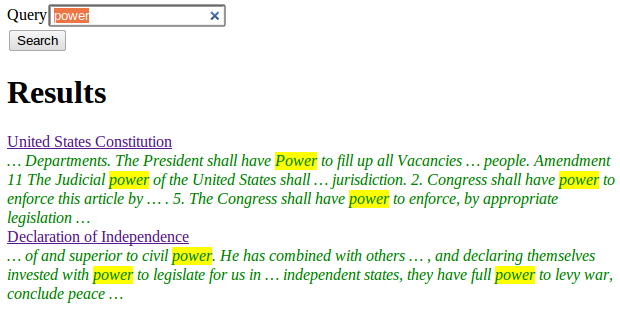
\includegraphics{21-search-results.png} % Результаты поиска (картинка)

Давайте начнем с определения типа данных Result:

\begin{lstlisting}
data Result = Result
    { resultId :: DocId
    , resultTitle :: Text
    , resultExcerpt :: Html
    }
\end{lstlisting}

Теперь взглянем на обработчик запроса поиска: % не поисковый запрос, ибо так переводится search term

\begin{lstlisting}
getSearchR :: Handler RepHtml
getSearchR = do
    ((formRes, searchWidget), _) <- runFormGet searchForm
    searchResults <-
        case formRes of
            FormSuccess qstring -> getResults qstring
            _ -> return []
    defaultLayout $ do
        toWidget [lucius|
.excerpt {
    color: green; font-style: italic
}
.match {
    background-color: yellow;
}
|]
        [whamlet|
<form method=get action=@{SearchR}>
    ^{searchWidget}
    <input type=submit value=Search>
$if not $ null searchResults
    <h1>Results
    $forall result <- searchResults
        <div .result>
            <a href=@{DocR $ resultId result}>#{resultTitle result}
            <div .excerpt>#{resultExcerpt result}
|]
\end{lstlisting}%$

Ничего волшебного здесь не происходит: мы просто полагаемся на \lstinline'searchForm', объявленную выше, и еще не объявленную \lstinline'getResults'. Эта функция просто принимает строку с поисковым запросом и возвращает список результатов. Здесь мы впервые взаимодействуем с API сервера Sphinx. Мы будем использовать две функции --- \lstinline'query' будет возвращать список совпадений, а \lstinline'buildExcerpts' --- выделенные отрывки. Взглянем на функцию \lstinline!query!:

\begin{lstlisting}
getResults :: Text -> Handler [Result]
getResults qstring = do
    sphinxRes' <- liftIO $ S.query config "searcher" (unpack qstring)
    case sphinxRes' of
        ST.Ok sphinxRes -> do
            let docids = map (Key . PersistInt64 . ST.documentId) $
                           ST.matches sphinxRes
            fmap catMaybes $ runDB $ forM docids $ \docid -> do
                mdoc <- get docid
                case mdoc of
                    Nothing -> return Nothing
                    Just doc -> liftIO $ Just <$>
                                  getResult docid doc qstring
        _ -> error $ show sphinxRes'
  where
    config = S.defaultConfig
        { S.port = 9312
        , S.mode = ST.Any
        }
\end{lstlisting}%$

Она принимает три аргумента : параметры конфигурации, строку с именем индекса, по которому будет производиться поиск, и поисковый запрос. Функция возвращает список идентификаторов документов, содержащих поисковый запрос. Здесь есть небольшая хитрость, связанная с тем, что возвращаемые идентификаторы имеют тип \lstinline'Int64', в то время как нам нужен \lstinline'DocId'. Благодаря тому, что SQL-бэкенды \lstinline'Persistent' используют конструктор \lstinline'PersistInt64' для этих идентификаторов, мы сможем получить требуемые значения.

\begin{remark}
  Если вы работаете с бэкендом, использующим нечисловые идентификаторы, например MongoDB, вам придется разработать какой-нибудь более изощрённый способ.
\end{remark}

Затем мы проходим в цикле по этим идентификаторам, получая список \lstinline'[Maybe Result]', и используем функцию \lstinline'catMaybes' для преобразования этого списка в \lstinline'[Result]'. В where-клозе мы определяем локальные настройки, которые замещают номер порта, используемый по умолчанию, а также задают режим поиска, в котором возвращаются все документы, содержащие хотя бы одно слово из поискового запроса. % "set up the search to work when any term matches the document" + в исходниках S.mode = ST.Any + см http://sphinxsearch.com/docs/1.10/matching-modes.html

Наконец, взглянем на функцию \lstinline'getResult':

\begin{lstlisting}
getResult :: DocId -> Doc -> Text -> IO Result
getResult docid doc qstring = do
    excerpt' <- S.buildExcerpts
        excerptConfig
        [T.unpack $ escape $ docContent doc]
        "searcher"
        (unpack qstring)
    let excerpt =
            case excerpt' of
                ST.Ok bss -> preEscapedToMarkup $ decodeUtf8With ignore $ L.concat bss
                _ -> ""
    return Result
        { resultId = docid
        , resultTitle = docTitle doc
        , resultExcerpt = excerpt
        }
  where
    excerptConfig = E.altConfig { E.port = 9312 }

escape :: Textarea -> Text
escape =
    T.concatMap escapeChar . unTextarea
  where
    escapeChar '<' = "&lt;"
    escapeChar '>' = "&gt;"
    escapeChar '&' = "&amp;"
    escapeChar c   = T.singleton c
\end{lstlisting}

Функция \lstinline'buildExcerpts' принимает четыре аргумента: параметры конфигурации, содержимое документа, строку с именем индекса и поисковый запрос. Обратите внимание на эранирование специальных символов в документе. Sphinx его не производит, поэтому нам приходится заниматься этим самим.

Результат поиска, который мы получаем от Sphinx, представляет собой список ленивых ByteString'ов. Но мы, само собой разумеется, предпочли бы получить \lstinline'Html'. Поэтому мы конкатенируем элементы списка в одну ленивую \lstinline'ByteString', декодируем ее в ленивый текст (игнорируя некорректные последовательности символов UTF-8), а затем используем функцию \lstinline'preEscapedToMarkup' для того, чтобы тэги, используемые для выделения найденных совпадений, не экранировались. Вот пример полученного в итоге HTML-кода:

\begin{lstlisting}[language=HTML]
&#8230; Departments.  The President shall have <span
class='match'>Power</span> to fill up all Vacancies
&#8230;  people. Amendment 11 The Judicial <span
class='match'>power</span> of the United States shall
&#8230; jurisdiction. 2. Congress shall have <span
class='match'>power</span> to enforce this article by
&#8230; 5. The Congress shall have <span
class='match'>power</span> to enforce, by appropriate legislation
&#8230;
\end{lstlisting}

\section{Генерируем xmlpipe} % Streaming xmlpipe output

Самое интересное мы приберегли напоследок. Для большинства обработчиков в Yesod рекомендуемый подход заключается в загрузке данных из базы в оперативную память и генерации вывода, основанного на этих данных. Так проще, но намного важнее то, что такой подход более устойчив к ошибкам.  Если возникнет проблема во время загрузки данных из базы, пользователь получит должный код ответа 500.

\begin{remark}
  Что я имею ввиду, говоря <<должный код ответа 500>>? Если вы начнете передавать данные клиенту и в середине процесса наткнетесь на исключение, у вас не будет возможности изменить код ответа. Пользователь получит ответ с кодом 200, просто передача данных прервется посередине. Помимо того, что частично сгенерированная страница сама по себе сбивает с толку, такое поведение еще и не соответсвтует спецификации протокола HTTP.
\end{remark}

Генерация xmlpipe-вывода является прекрасным примером, где следует использовать альтернативный подход. У нас может быть огромное количество документов (код сайта yesodweb.com оперирует десятками тысяч документов), а документы могут иметь размер порядка нескольких сотен килобайт. Если мы не воспользуемся поточным подходом, это может привести к большому времени ответа и использованию большого объёма оперативной памяти.

Так каким именно образом мы можем сгенерировать ответ в виде потока? %streaming response
Как мы узнаем из \hyperref[chap:web_application_interface]{главы, посвященной WAI}, у нас есть конструктор \lstinline!ResponseSource!, который использует поток элементов типа \lstinline!Builder! из библиотеки \lstinline'blaze-builder'. На стороне Yesod, вместо того, чтобы генерировать ответ, как обычно, мы можем послать WAI-ответ напрямую с помощью функции \lstinline'sendWaiResponse'. Таким образом имеется по крайней мере две части этой головоломки. % So there are at least two of the pieces of this puzzle.

Теперь нам известно, что из неких XML-данных требуется создать поток Builder'ов. К счастью, пакет \footnotehref{http://hackage.haskell.org/package/xml-conduit}{\lstinline'xml-conduit'} предоставляет интерфейс непосредственно для этого. Вообще пакет \lstinline'xml-conduit' предоставляет высокоуровневый интерфейс для работы с документами целиком, однако в нашем случае понадобится низкоуровневый интерфейс Event, дабы обеспечить минимальное использование памяти. Вот функция, которая нам нужна:

\begin{lstlisting}
renderBuilder :: Resource m => RenderSettings -> Conduit Event m Builder b
\end{lstlisting}

В переводе на русский язык это означает, что renderBuilder принимает некие настройки (мы воспользуемся настройками по умолчанию), и преобразует поток \lstinline!Event!'ов в поток \lstinline!Builder!'ов. Выглядит неплохо. Все, что нам теперь нужно --- это поток \lstinline!Event!'ов.

Кстати говоря, а как должен выглядеть наш XML-документ? Он довольно прост, имеется родительский элемент \lstinline'sphinx:docset', элемент \lstinline'sphinx:schema', содержащий одиночный элемент \lstinline'sphinx:field' (который определяет элемент с содержимым документа), а затем по одному элементу \lstinline'sphinx:document' для каждого документа в базе данных. Эти элементы будут содержать атрибут id и дочерний элемент \lstinline'content'.

\begin{remark}
Пример xmlpipe-документа % Sample xmlpipe document - TODO в исходнике это заголовок (title), возможно надо как-то отформатировать в tex тоже?
\begin{lstlisting}[language=XML]
<sphinx:docset xmlns:sphinx="http://sphinxsearch.com/">
    <sphinx:schema>
        <sphinx:field name="content"/>
    </sphinx:schema>
    <sphinx:document id="1">
        <content>bar</content>
    </sphinx:document>
    <sphinx:document id="2">
        <content>foo bar baz</content>
    </sphinx:document>
</sphinx:docset>
\end{lstlisting}
\end{remark}

Каждый XML-документ будет начинатся с одинаковых событий (начать docset, начать schema и т.д.) и заканчиваться одним и тем же событием (закончить docset). Вот соответствующий код: % We'll start off by defining those:

\begin{lstlisting}
toName :: Text -> X.Name
toName x = X.Name x (Just "http://sphinxsearch.com/") (Just "sphinx")

docset, schema, field, document, content :: X.Name
docset = toName "docset"
schema = toName "schema"
field = toName "field"
document = toName "document"
content = "content" -- no prefix

startEvents, endEvents :: [X.Event]
startEvents =
    [ X.EventBeginDocument
    , X.EventBeginElement docset []
    , X.EventBeginElement schema []
    , X.EventBeginElement field [("name", [X.ContentText "content"])]
    , X.EventEndElement field
    , X.EventEndElement schema
    ]

endEvents =
    [ X.EventEndElement docset
    ]
\end{lstlisting}

Теперь, когда у нас есть оболочка нашего документа, нам нужно достать \lstinline!Event!'ы для каждого конкретного документа. Это можно сделать при помощи довольно простой функции:

\begin{lstlisting}
entityToEvents :: (Entity Doc) -> [X.Event]
entityToEvents (Entity docid doc) =
    [ X.EventBeginElement document [("id", [X.ContentText $ toPathPiece docid])]
    , X.EventBeginElement content []
    , X.EventContent $ X.ContentText $ unTextarea $ docContent doc
    , X.EventEndElement content
    , X.EventEndElement document
    ]
\end{lstlisting}
%TOCONTINUE
Мы начинаем с элемента document, имеющего атрибут id, затем начинаем элемент content, вставляем содержимое документа, после чего закрываем оба элемента. Для преобразования \lstinline!DocId! в значение типа \lstinline!Text! мы используем функцию \lstinline!toPathPiece!. Теперь нам нужно как-то преобразовать поток сущностей в поток событий. Для этого воспользуемся функцией \lstinline!concatMap! из модуля \lstinline!Data.Conduit.List!: \lstinline`CL.concatMap entityToEvents`.

Но чего мы \emph{действительно} хотим, так это создать поток этих событий непосредственно из базы данных. На протяжении большей части книги, мы использовали функцию \lstinline!selectList!, однако Persistent также предоставляет (более мощную) функцию \lstinline!selectSourceConn!. С ее помощью мы получаем в итоге следующую функцию: % So we end up with the function:

\begin{lstlisting}
docSource :: Connection -> C.Source (C.ResourceT IO) X.Event
docSource conn = selectSourceConn conn [] [] C.$= CL.concatMap entityToEvents
\end{lstlisting}%$

Оператор \$= соединяет источник с каналом, возвращая новый источник. Теперь, когда у нас есть источник \lstinline!Event!'ов, все, что нам нужно --- это окружить его событиями начала и конца документа. Благодаря тому, что Source является экземпляром класса \lstinline!Monoid!, это проще простого:

\begin{lstlisting}
fullDocSource :: Connection -> C.Source (C.ResourceT IO) X.Event
fullDocSource conn = mconcat
    [ CL.sourceList startEvents
    , docSource conn
    , CL.sourceList endEvents
    ]
\end{lstlisting}

Мы почти закончили, осталось только применить все это в функции \lstinline!getXmlpipeR!. Нам необходимо установить соединение с базой данных. Обычно соединения с БД берутся и автоматически возвращаются с помощью функции \lstinline!runDB!. В нашем случае требуется получить соединение и иметь к нему доступ до тех пор, пока тело ответа не будет передано полностью. Для этого воспользуемся функцией \lstinline!takeResource!, которая регистрирует действие по очистке в монаде \lstinline!ResourceT!.

\begin{remark}
Все WAI-приложения живут в трансформаторе монады \lstinline!ResourceT!. Вы можете получить больше информации о \lstinline!ResourceT! в \hyperref[chap:conduit]{приложении, посвященном потокам}.% (conduit)
\end{remark}

По умолчанию ресурс не возвращается в пул. Это связано с правильной обработкой ошибок, что, впрочем, не относится к нашему случаю. Поэтому мы должны принудительно вернуть соединение в пул:

\begin{lstlisting}
getXmlpipeR :: Handler RepXml
getXmlpipeR = do
    Searcher pool <- getYesod
    let headers = [("Content-Type", "text/xml")]
    managedConn <- lift $ takeResource pool
    let conn = mrValue managedConn
    lift $ mrReuse managedConn True
    let source = fullDocSource conn C.$= renderBuilder def
    sendWaiResponse $ ResponseSource status200 headers source
\end{lstlisting}

Пул соединений получается из базовой переменной, после чего отправляется WAI-ответ. Мы используем конструктор \lstinline!ResponseSource!, передавая ему код ответа, а также заголовки и тело ответа.

\section{Весь код} % Full code

\lstinputlisting{../hs/21-source.hs}
